\documentclass[12pt]{article}
\usepackage[utf8]{inputenc}
\usepackage[T1]{fontenc}
\usepackage[spanish]{babel}
\usepackage{amsmath, amssymb}
\usepackage{geometry}
\usepackage{graphicx}
\usepackage{url}
\usepackage{float}
\usepackage{caption}
\usepackage{subcaption}
\usepackage{hyperref}
\usepackage{cite}
\usepackage{wrapfig}
\geometry{a4paper, margin=1in}

\title{Nuevo sistema y precisión}
\author{Alan David Rodríguez Cruz\\ 20252020082 \\ Josué Nicolás Riascos Pizarro \\ 20252020084 \\ Samuel Andrés Rojas Escobar \\ 20252020077 \\ Universidad Distrital Francisco José de Caldas}
\date{2025}



\begin{document}

\maketitle

\section*{Resumen}
En este texto se busca evidenciar si se puede crear un nuevo sistema de medida preciso que permita solucionar la incógnita del área de una figura en una hoja cuadriculada considerando las dimensiones de los cuadrados que la contienen y cuáles serían los cálculos matemáticos más adecuados para ello utilizando textos de referencia como: \textit{Demostración de la fórmula clásica para calcular el área de un triángulo (base por altura sobre dos) mediante la geometría analítica y el cálculo integral} por José de Jesús Camacho y \textit{Precálculo: Matemáticas para el cálculo (6ª ed.)} de James Stewart.

\section*{Introducción}
El propósito de este experimento es calcular el área de una figura compuesta por triángulos, rectángulos y una figura parabólica. Para esto se utiliza como base una hoja cuadriculada que permite establecer un sistema de unidades propio mediante la relación entre cuadros grandes y cuadros pequeños.

\section{Descripción del experimento y mediciones}
\subsection{Materiales}

\begin{itemize}
    \item Hoja guía \\
    \includegraphics[width=0.25\linewidth, angle=90]{Experimento1_page-0001.jpg}

    \item Lápiz \\
    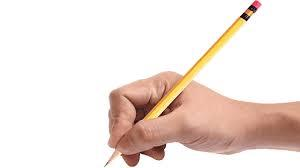
\includegraphics[width=0.25\linewidth]{page2_img2.jpeg}

    \item Regla \\
    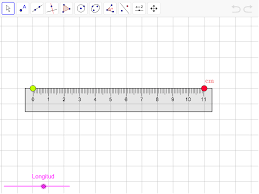
\includegraphics[width=0.25\linewidth]{page2_img3.png}
\end{itemize}

Se observa la imagen de la hoja guia e inmediatamente se notan algunos puntos. Lo primero que se observa es que no hay una unidad de medida especificada; para resolver esto, el equipo distingue cierta representación en cuadros donde unos son más grandes y contienen otros más pequeños. En vista de lo anterior, el equipo decidió asignarle los siguientes nombres para que sea más práctico representarlos después. 

\begin{itemize}
  \item Cuadros más grandes = $A$
  \item Cuadros más pequeños = $a$
\end{itemize}

También se pudo notar que existe la siguiente relación entre $A$ y $a$:

Dentro de cada $A$ hay $100a$, por lo que podemos decir que:

\[ A^2 = 10a^2 \]

Después, el equipo busca similitudes en el sistema de unidades métrico decimal (en concreto los centimetros). Para ello se utilizó una regla y se encontró qué el cuadro "A” no mide exactamente 1 cm, aunque si es bastante cercano por lo que se tuvo en cuenta para comparar con el fin de que se pudiera ver una relación entre la cantidad de cuadros (“A” y “a”) y los centímetros que representan el área total de la figura. 

Se encontró que la Longitud total de la figura es de 22A o 220a lo que permitió calcular áreas de manera aparentemente precisa, incluso sin usar una medición real en centímetros. También para su altura se contaron 14A o 140a por lo que teniendo en cuenta lo que dice Camacho (2019) que se forman 2 triángulos al trazar una diagonal en un rectángulo, donde al tener la formula clásica del área de un triángulo 
\[ A = {\frac{bh}{2}} \]
Donde b es la base y h la altura, se puede afirmar que el área de un rectángulo es 
\[A = {2*\frac{bh}{2}} = bh\]

O dicho de otra manera el área de un rectángulo es el producto de su base por su altura. 

La longitud total de la figura es de $22A$ o $220a$ y la altura es de $14A$ o $140a$.

\section{Cálculo de áreas}
\subsection{Rectángulo exterior}

\begin{figure}[H]
    \centering
    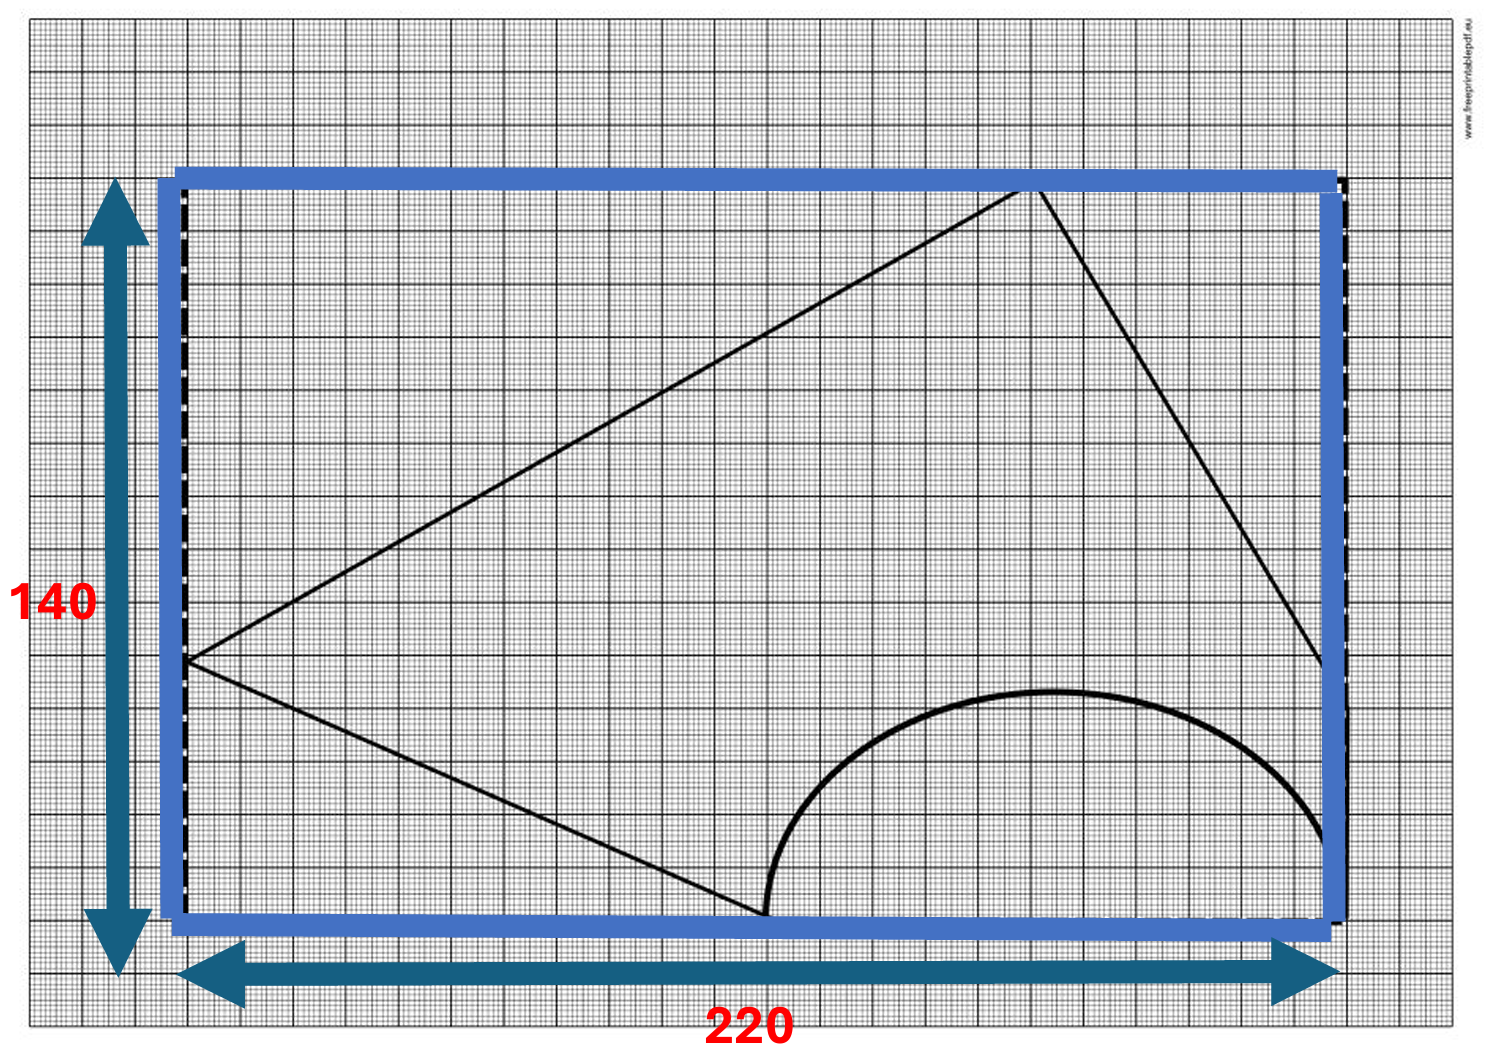
\includegraphics[width=0.5\linewidth]{imagen 1.png}

\end{figure}    

\begin{align*}
A_\text{rect} &= 22A \cdot 14A \approx 308A \\
A_\text{rect} &= 220a \cdot 140a \approx 30800a
\end{align*}
Ya teniendo el área del rectángulo exterior se busca el área de los triángulos interiores además con la ecuación del área de un círculo que aparece en las páginas de referencia del libro “cálculo de una variable” (Stewart, 2012) donde el área de un círculo es:
\[A = {\pi r^2}\]
Por lo que podemos afirmar que el área de un semicirculo es:


\[A = {\frac{\pi r^2}{2}}\]

Donde $\pi$ es un valor constante que siempre relaciona la circunferencia con el diámetro y $r$ es el valor desde el centro de la circunferencia hasta su borde (radio).



\subsection{Triángulos interiores}

\begin{figure}[H]
    \centering
    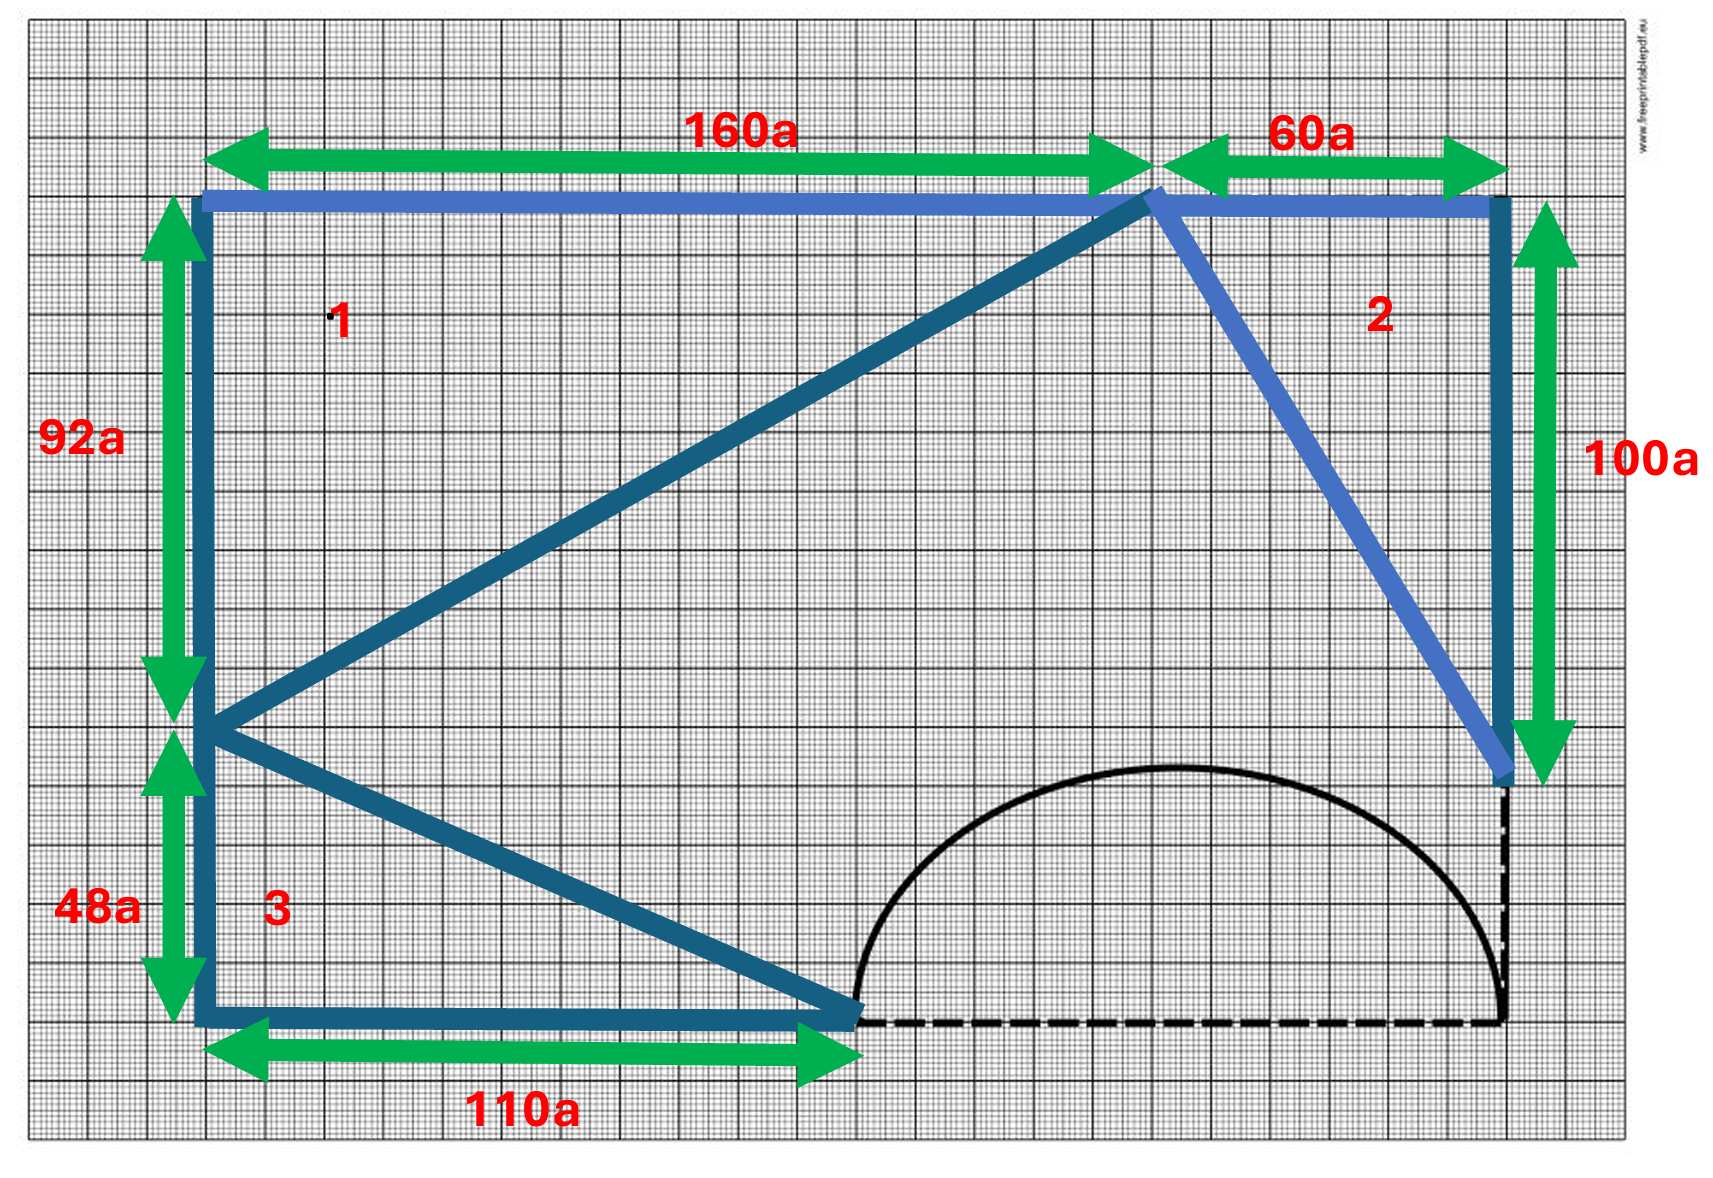
\includegraphics[width=0.5\linewidth]{imagen 2.png}
\end{figure}

\begin{align*}
A_{T1} &= \frac{92a \cdot 160a}{2} \approx 7360a \\
A_{T2} &= \frac{60a \cdot 100a}{2} \approx 3000a \\
A_{T3} &= \frac{48a \cdot 110a}{2} \approx 2640a
\end{align*}

\subsection{Semicírculo}

Ahora calculamos el área del semi circulo que está en la parte inferior de la figura.

\begin{figure}[H]
    \centering
    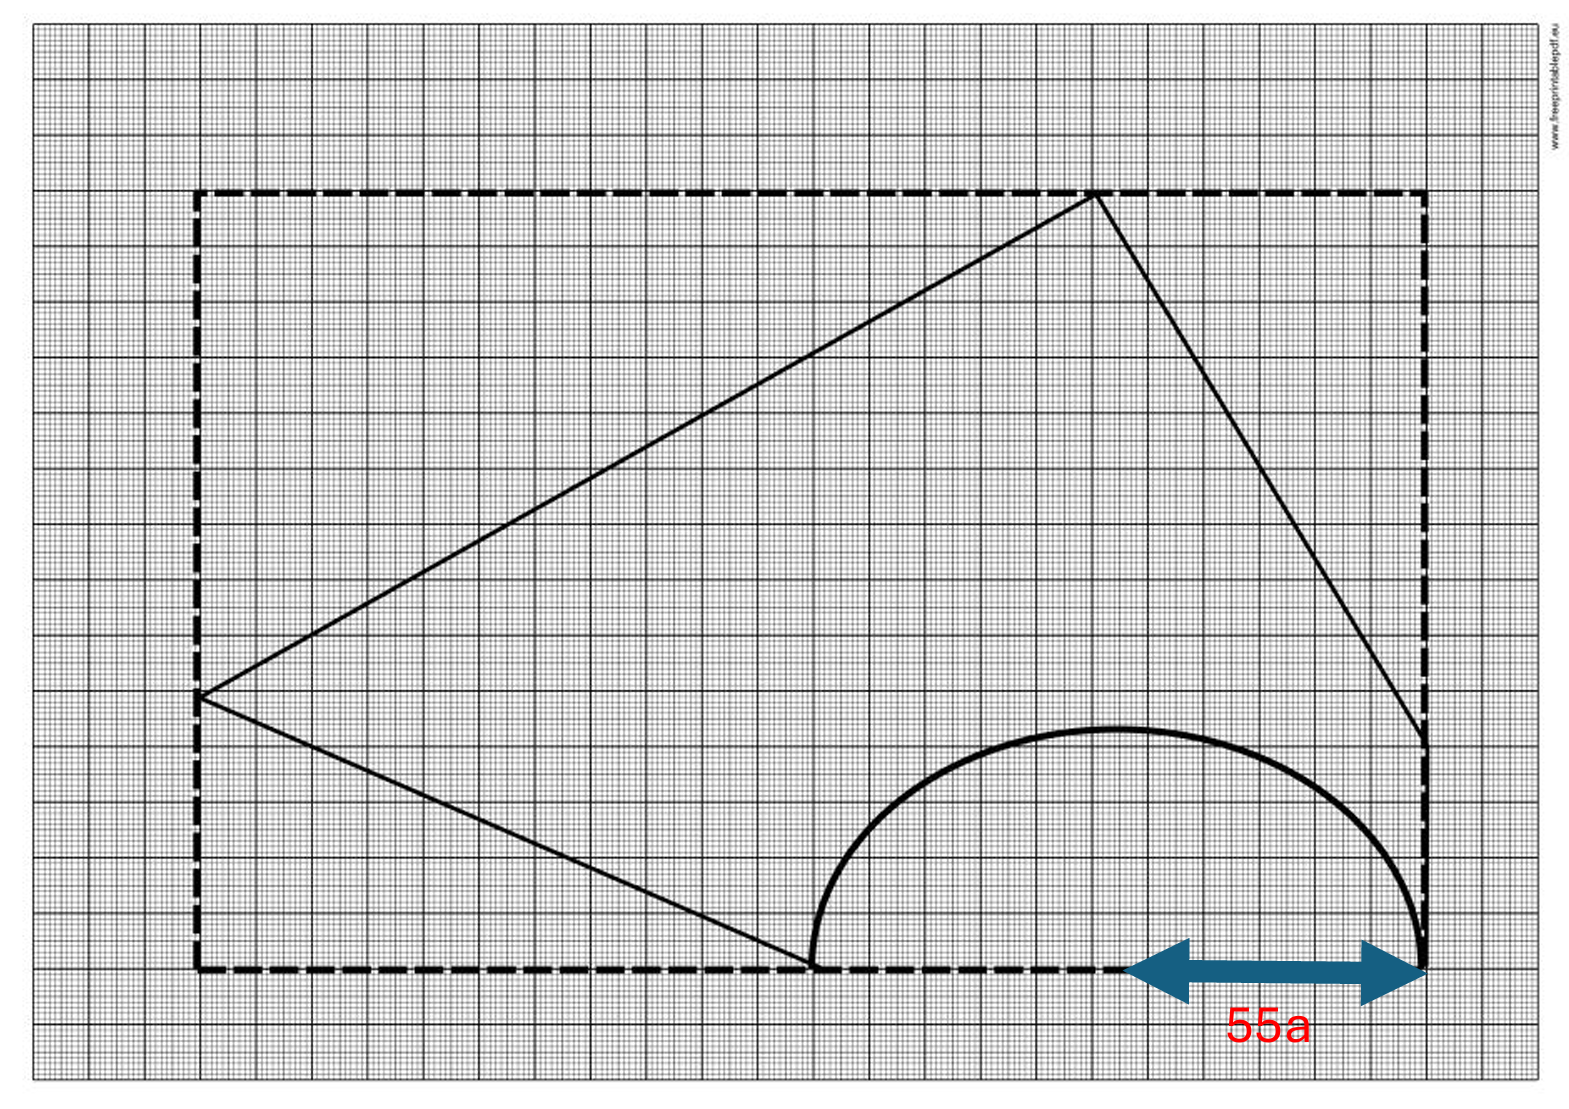
\includegraphics[width=0.5\linewidth]{imagen 3.png}

\end{figure}

\begin{align*}
A_C &= \frac{\pi (55a)^2}{2} \approx 4751.65a
\end{align*}



\subsection{Área final}

Ya teniendo el área de los 3 triángulos y el semi circulo el equipo decide restar la sumatoria de las áreas de los 3 triángulos y la del semi circula al área total del rectángulo exterior.  Por lo que se ve como una ecuación de este estilo: 

\begin{align*}
A_\text{fig} &= A_\text{rect} - (A_{T1} + A_{T2} + A_{T3}) - A_C \\
A_\text{fig} &= 30800a - (7360a + 3000a + 2640a) - 4751.65a \\
A_\text{fig} &\approx 13048.35a
\end{align*}

Teniendo en cuenta todo lo anterior se puede afirmar que el área total de la figura es equivalente a 13048,35a. 

\section*{Conclusiones}
En conclusión, si bien se pudieron realizar los cálculos y las mediciones para realizar la estimación del área de la figura, dado que la medida que invento el equipo de “A” y “a” es cercana al centímetro, es imposible determinar con exactitud a cuanto equivale un “A” o un “a” en centímetros o en cualquier otro sistema métrico más o menos preciso, ya que los “A” y los ”a” dependen de factores externos como el tamaño de la impresión, la calidad de esta, la calidad de la hoja u muchos otros que lo hacen una medida que no es para nada precisa ni recomendable de usar en circunstancias reales, además es menester tener en cuenta que para calcular inicialmente el tamaño de las dimensiones que en este texto llamamos “A” y “a” a centímetros siempre había que dejar un margen de ± 0.5 centímetros, por lo que también afecta a la medición de un sistema más preciso como puede ser el uso de los centímetros. 
\begin{thebibliography}{9}
\bibitem{camacho2019}
Camacho Medina, J. de J. (2019). \textit{Demostración de la fórmula clásica para calcular el área de un triángulo (base por altura sobre dos) mediante la geometría analítica y el cálculo integral.} Revista MasScience. \url{https://www.masscience.com/2019/02/21/demostracion-de-la-formula-clasica-para-calcular-el-area-de-un-triangulo-base-por-altura-sobre-dos-mediante-la-geometria-analitica-y-el-calculo-integral/}

\bibitem{stewart2012}
Stewart, J. (2012). \textit{Precálculo: Matemáticas para el cálculo} (6ª ed.). Cengage Learning.
\end{thebibliography}

\end{document}
